
\section{Evaluation}
\label{sec:evaluation}
This section evaluates the % performance of \specula when deployed over We deployed \specula over nine geo-distributed datacenters (DCs) of Amazon EC2 and evaluated it using both synthetic workloads and realistic benchmarks, namely TPC-C and RUBiS. We report the 
 performance achievable by \specula when using exclusively internal speculation, i.e., speculative reads, and when enabling also external speculation, in which case speculative commits are immediately externalized to clients. In the following, we refer to the first \specula's variant as to  {\specula}-Internal, and to the second one as {\specula}-External. This choice allows us to contrast the performance achievable by \specula when speculation is used in a fully transparent way for the application, with the case in which programmers are willing to incur the risk of exposing mispeculations to clients.% and to develop compensation logic to cope with them.

%Recall that the use of external speculation  allows us to evaluate the performance achievable 
%
%, which allow us to generate workloads 
%
%a synthetic workload and two realistic applications, namely TPC-C and RUBiS. The evaluation includes two variations of our STR, one that only performs speculative read ({\specula}-Internal) and one that can perform both speculative read and speculative commit ({\specula}-External), against two transactional protocols. The results show that even without externalizing speculative results, we can achieve about 3.5$\times$ speedup for workloads with high local contention and low remote contention. Nevertheless, allowing speculative commit can further reduce latency by XXX. \textbf{How to write latency reduction? For some workload, our final latency is 300 while the baselin is 21000, so we say by a factor or 70? What about for perceived latency?}

%\subsection{\specula variations and baselines}
%We implemented two variations of \specula, namely {\specula}-Internal and  {\specula}-External. {\specula}-Internal only allows speculative read, which means it does not externalize speculative results (with respect to 'internal') and does not require writing compensation logic; on the other hand, {\specula}-External allows both speculative read and speculative commit, which may externalize speculative results. Both protocols are run with an automatic tuning process. The automatic tuning process collects throughput statistics from all servers every twenty seconds \textbf{should I mention that?}, then it calculates the next speculation level and informs all servers. The tuning starts with the most conservative speculation level, i.e. no speculative read and no speculative commit, then proceeds until it finds a speculation level that gives the maximal throughput. The possible speculation levels, from conservative to aggressive, are: no speculative read (No SR), only speculative read (SR, the maximal level {\specula}-Internal can have), speculative read and speculative commit with length one (SR+SL1), ..., till SR+SL8 (the maximal level {\specula}-External can have).

Unless otherwise specified, both \specula variants use the hill-climbing self-tuning mechanism described in \S~\ref{subsec:tuning}. For the case of {\specula}-Internal, the self-tuning mechanism simply determines whether to use or not speculative reads. With {\specula}-External, conversely, the self-tuning mechanism also determines whether, in addition to using speculative reads, also speculative commits should be used and the maximum length, in the [1,8] range, of the speculation chain length.


We use two baseline protocols. The first one employs ClockSI~\cite{clocksi}, a non-speculative  transactional protocol that, like \specula, provides Snapshot Isolation using a decentralized timestamp-based concurrency control mechanism. As the original ClockSI protocol does not support replication, in order to ensure a fair comparison with \specula, we extended it to use the same primary-backup replication mechanism employed by \specula. We refer to this protocol as to ClockSI-Rep. The second baseline aims to emulate protocols, like PLANET \cite{pang2014planet}, which allows for externalizing  to clients  the results of transactions that pass their local certification phase. Unlike \specula, though, PLANET does not allow speculative reads nor supports pipelining of speculative transactions, i.e., clients cannot activate new transactions before final committing any previously speculatively committed transaction. PLANET was originally layered on top of MDCC~\cite{mdcc}, which only supports full data replication. In order to ensure an apple-to-apple comparison with the remaining protocols considered in our study, we implement this baseline by building it atop ClockSI-Rep and allowing each client to speculatively commit one transaction.

% while not allowing speculative read or pipelining speculative transactions. As in the original paper, PLANET is built on top of the MDCC protocol \cite{kraska2013mdcc} and uses a prediction model to decide whether to speculate. Since it is not possible to do an apple-to-apple comparison, we implemented a simplified version of PLANET, by building it atop ClockSI-Rep and additionally allows each client to speculatively commit one transaction. 

\subsection{Experimental setup}
\label{subsec:setup}
We implemented our baseline protocol and \specula in  Erlang, based on \textit{antidote}, a popular open-source platform for evaluating distributed consistency protocols \cite{antidote}.

The system is deployed across the following nine DCs of Amazon EC2: Ireland(IE), Seoul(SU), Sydney(SY), Oregon(OR), Singapore(SG), North California(CA), Frankfurt(FR),  Tokyo(TY) and North Virginia(VA). Each DC consists of three m4.large instances (2 VCPU and 8 GB of memory) and each instance holds the master replica of one partition.  DCs are arranged in a consistent hashing ring according to the order of the above list; each partition is replicated across the five DCs that follow the DCs hosting the master replica of that partition, e.g., 
 the  partitions whose primary replicas are maintained at the CA datacenter are replicated by the 
 FR, TY, VA, IE and SU DCs. %Table~\ref{tab:latency} reports the largest network latencies incurred at the various data centers to contact one of its replicas and any other data center in the cluster.
 
%  We interleave DCs from nearby regions in the consistent hash ring, so to reduce the variance in the replication  latencies incurred by different  data centers.
 
% hat different replication groups will have similar latency to perform replication, as shown in table \ref{tab:latency}.

A workload stressor is located at each node of the system, which spawns one thread per emulated client. Each client issues transactions to a pool of local transaction coordinators and retries a transaction if it gets aborted. We use two metrics to evaluate latency: the \textit{final latency} of a transaction is calculated as the time elapsed since the first activation of a transaction  until its final commit (including possible aborts and retries); the \textit{perceived latency} is defined as the time since the first activation of a transaction until its last speculative commit event, i.e., the one after which it is finally committed. Each reported result is obtained  from the average of at least three runs. We omit reporting standard deviations in the plots to enhance their readability, and since they were always lower than 10\% than the reported mean values.

%duration from its first trial to its commit time, and the user perceived latency (for speculative commit) is measured as the duration from its first trial to its last speculative commit (after which it commits). Last but not least, each experiment is run for three times. We discard the aggregate results of the first twenty seconds and show the average value (deviation is low).

%\begin{table*}
%\small
%\begin{center}
%  \begin{tabular}{l |  l | l | l| l | l | l| l| l |l } 
%     & IE & SU& SY& OR & SG & CA &  FR & TY & VA  \\ \hline
%  \textbf{Max latency (replicas)} & 334(SG) & 267(FR) & 321(FR) & 160(SG)  & 337(IE) & 167(FR) & 321(SY)& 212(IE)  &  226(SY)  \\   \hline
%  \textbf{Max latency (all)} &  334(SG) &  267(FR) & 321(FR)  & 163(SY) & 337(IE) & 175(SG) & 324(SG)  & 233(FR)  & 226(SY) \\ \hline
%  \end{tabular}
%\end{center}
%\caption{Largest network latency experienced, on average, by a DC to contact any of its  replicas and any other DC (msec).}
%\label{tab:latency}
%\end{table*}

\subsection{Synthetic workloads}
We start by considering a synthetic benchmark, which allow us to to evaluate \specula's performance in presence of workloads with precisely identifiable and very heterogeneous characteristics.The synthetic benchmark generates transactions with null ``think time'', i.e., client threads issue a new transaction as soon as the previous one is final committed, for ClockSI-REP and {\specula}-Internal, or speculatively committed, for {\specula}-External and PLANET. As such, this benchmark is representative of non-interactive applications, in which transactions are used to support machine-to-machine interactions. (like, e.g., in high frequency trading applications).

%We 
% represent idealistic non-interactive workloads, where each thread issues a new transaction as soon as the previous one is committed (or speculative committed). In these experiments, we pick four representative contention levels to check the performance of these protocols.

\paragraph{Transaction and data access} A transaction reads 10 keys then updates them. When accessing a data partition, 90\% of the accesses goes to a small set of keys in that data partition, which we call a hotspot, and we adjust the size of the hotspot to control contention rate. Each data partition has two million keys, of which one million are only accessible by locally-initiated transactions and the others are only accessible by remote transactions. This allows adjusting in an independent way  the likelihood of contention among transactions initiated by the same local node (local contention) and among transactions originated at remote nodes (remote contention).

We consider four workload scenarios, which we obtain by varying the size of the hotspot size in the local and remote data partitions: i) low local and remote contention, ii) low local  and high remote contention, iii) high local and low remote contention, and iv) high local and remote contention.% We set the size of the local hotspot size

%In the following, we use a hotspot size of 30000 keys 

% denote 30000 keys for the size of local hotspot size as low local contention and 1000 keys as high local contention; according, 15000 keys for a remote hotspot is named low remote contention and 500 keys for high remote contention. 80\% of a transaction's key access goes to local master partitions, while 20\% goes to slave data partitions replicated locally.

\begin{figure*}
\centering
\def\svgwidth{0.98\columnwidth}
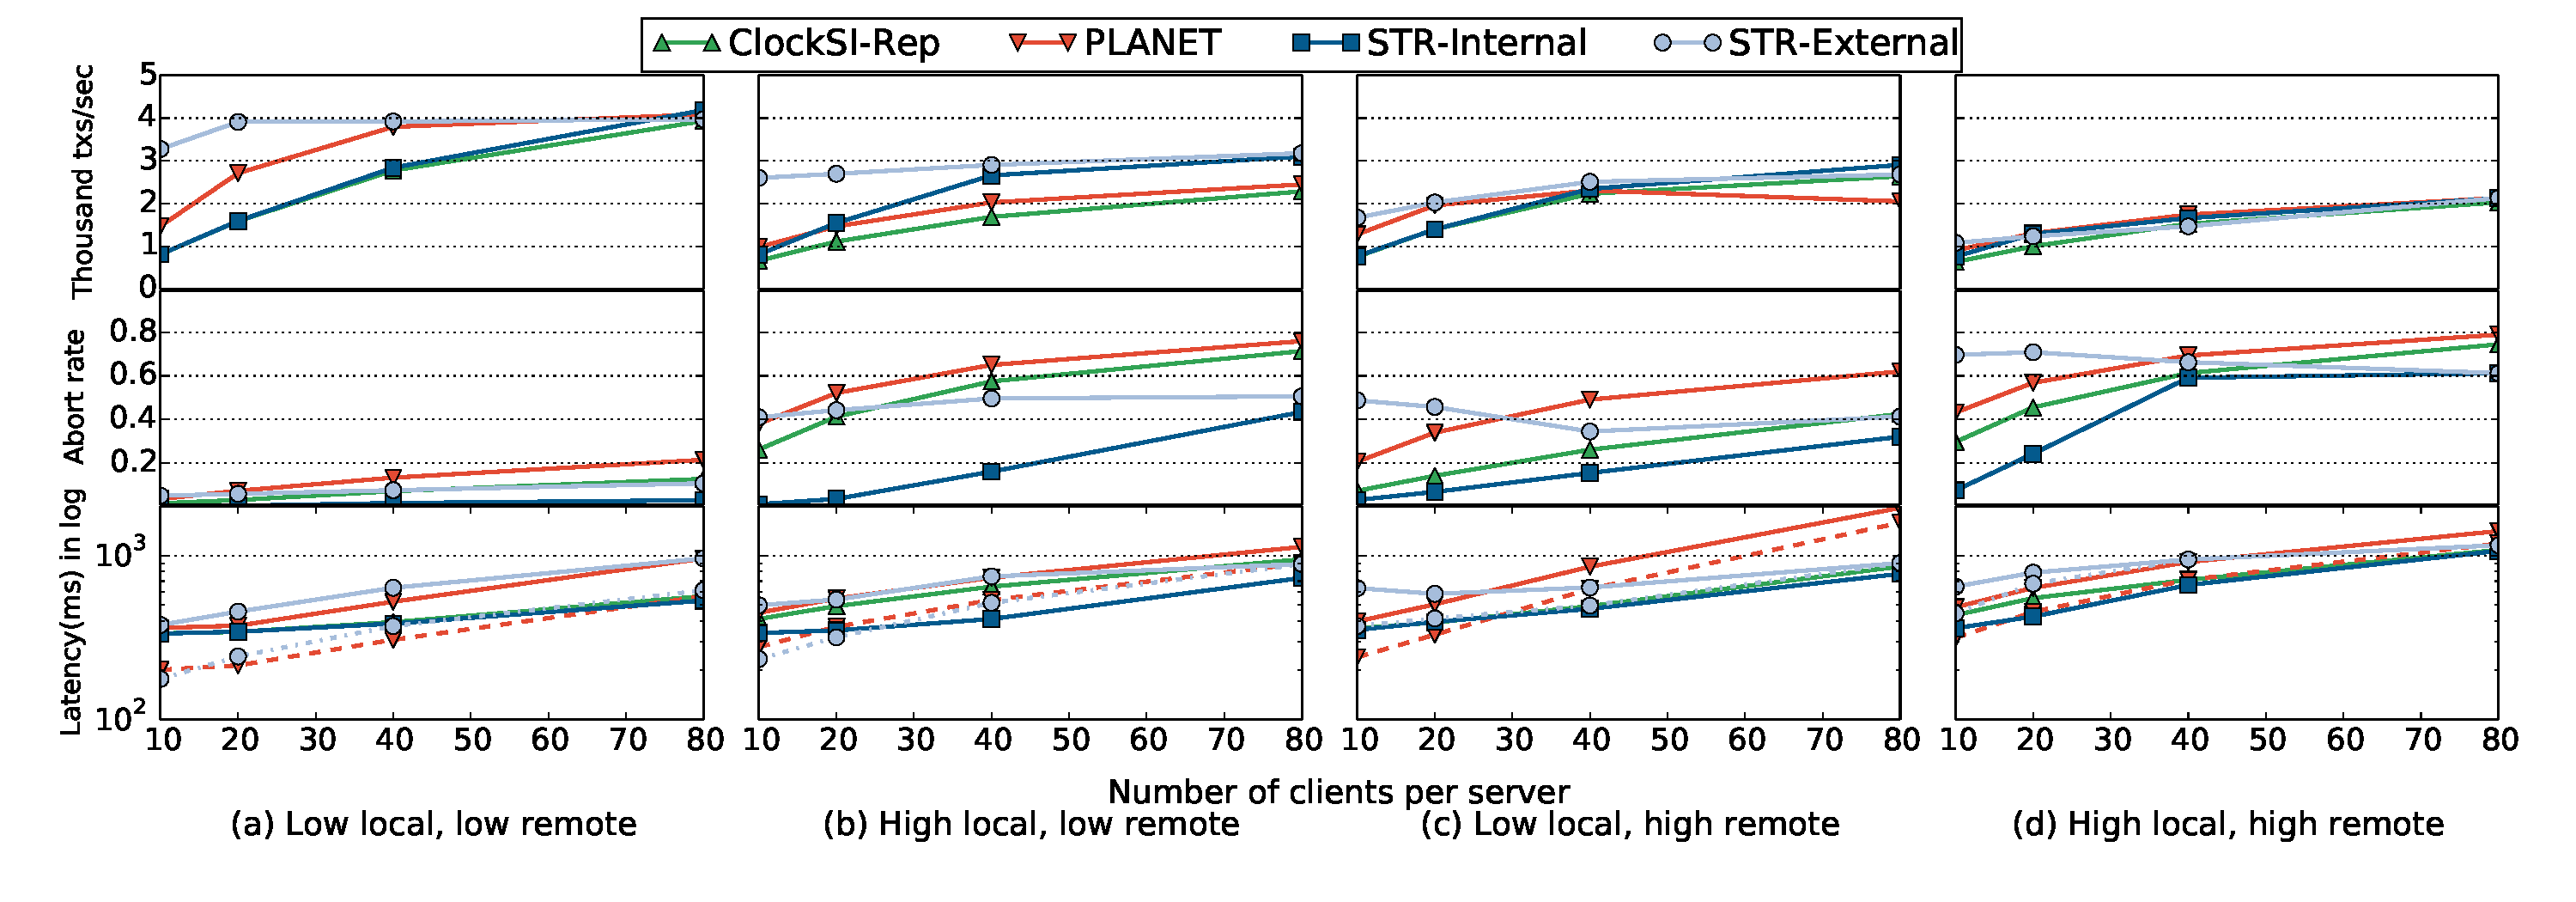
\includegraphics[scale=0.35]{figures/micro}
\vspace{-9mm}
\caption{\small \textit{Performance of different protocols under four levels of contention.} \textit{Low local, high remote} denotes low local contention and high remote contention, and so forth. In the latency plot, we use solid lines for final latency and dashed lines for  perceived latency.}
\label{fig:micro}
\end{figure*}


\begin{figure}[t]
\centering
\def\svgwidth{0.98\columnwidth}
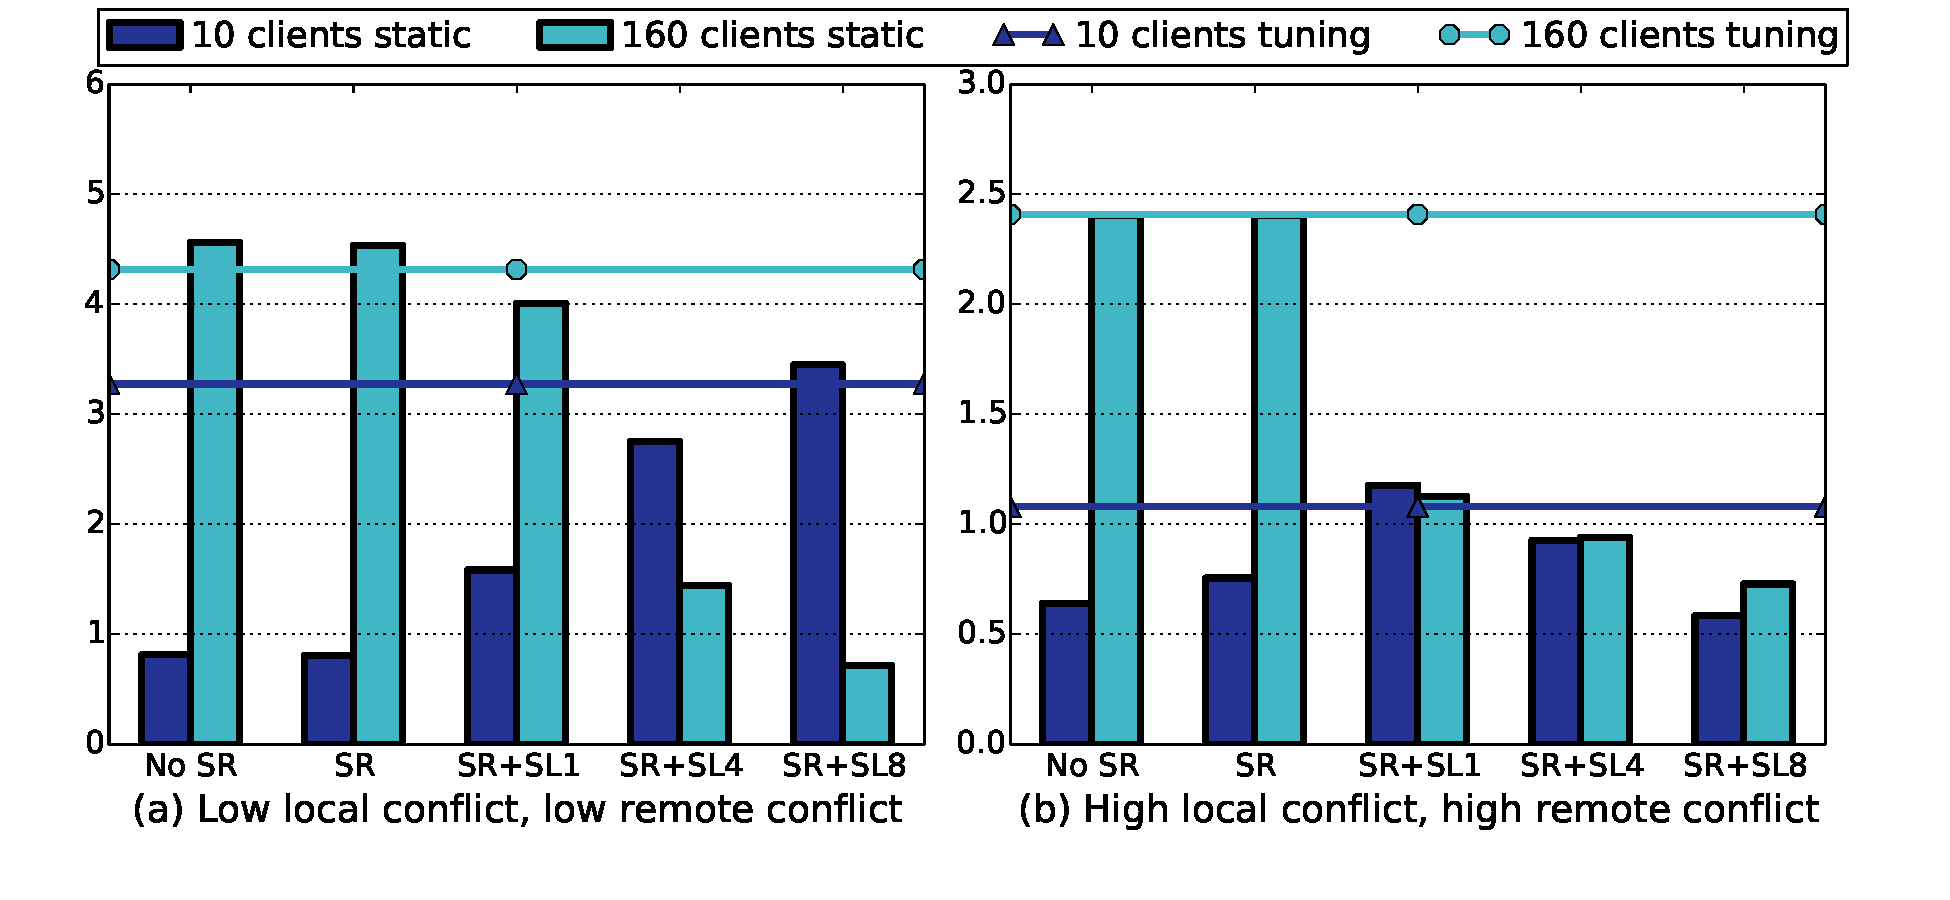
\includegraphics[scale = 0.28]{figures/tuning}
\vspace{-9mm}
\caption{\small The throughput of tuning versus static configuration}
\label{fig:tuning}
\end{figure}

\paragraph{Analysis of the results.} Let us start by considering a workload characterized by both low local contention and low remote contention. As shown in figure \ref{fig:micro}a, both PLANET and {\specula}-External achieve significantly higher throughput than ClockSI-REP when up to 40 clients are used. This can be explained by considering that, with these two protocols, clients can activate one (for the case of PLANET) or more (for the case of  {\specula}-External) new transactions, as soon as they have speculatively committed a transaction. With both ClockSI-REP and  {\specula}-Internal, instead, clients can only initiate a new transaction once they have final committed their previous transactions. In other words, with ClockSI-REP and  {\specula}-Internal, clients submit new transactions at a frequency that is equal to the inverse of the final latency, whereas, with PLANET and   {\specula}-External, the frequency of generation of new transactions is equivalent to the inverse of the perceived latency.

As we can see from the latency plot the perceived latency is about 4$\times$ smaller than the final latency in this workload, in which mispeculation are unlikely to occur given the low contention likelihood. It is worth noting that since {\specula}-External  can support the pipelining of multiple speculative transactions at a given client, this protocol achieves the peak throughput supported by the system (4K txs/sec) with about half of the clients that are required to saturate the system with PLANET (i.e., 20 vs 40 clients). Also, {\specula}-External achieves peak throuhgput gains of  4$\times$ and 2$\times$  when compared with ClockSI-REP and PLANET, respectively.

As the number of clients increases to 80 the use of external speculation in PLANET and {\specula}-External  continues to yield benefits in terms of latency. Yet, this does not reflect directly into a throughput increase vs ClockSI-REP and {\specula}-Internal: with such a large client population, both ClockSI-REP and {\specula}-Internal can fully utilize the available system's resources given that this workload generates very reduced data contention levels.
The  negligible contention generated by this workload creates also little chances of exploiting the speculative read technique, which explain why  {\specula}-Internal and ClockSI-REP achieve almost identical performance. Nonetheless, the use of the PreciseClock mechanisms allows  {\specula}-Internal to achieve a perceivable abort reduction at high load. As with this workload speculative reads are not effective (due to its negligible degree of contention), this experiment allows us to indirectly quantify the overheads introduced by the concurrency control mechanisms used by \specula to support internal speculation (i.e., speculative reads and PreciseClock). Indeed, the fact that the throughputs achieved by ClockSI-REP and  {\specula}-Internal in this workload are  indistinguishable represents an experimental evidence supporting the efficiency of the proposed mechanisms.


Figure \ref{fig:micro}b shows a workload with high local and low remote contention. This is a favourable workload for {\specula}-Internal and {\specula}-External. In fact, these protocols avoid blocking transactions that read pre-committed data records an, this workload, transactions that pass their local certification phase are likely to commit due to the low probability of remote contention. Since PLANET does not use speculative reads, instead, it is forced to frequently block transactions. This leads to an increase of the duration of the transaction execution phase, which makes transactions more vulnerable to conflicts and prone to abort.

As in the previous workload, the throughput gains of  {\specula}-External are particularly large (up to \~4$\times$) with a small number of clients, as this protocol utilizes more effectively than its competitors the available hardware resources thanks to its ability to pipeline successfully the execution of speculatively committed transactions. Unlike in the previous workload, though, both 
\specula variants achieve significant throughput gains also at high client counts, namely approximately 45\% at 40 and 80 clients. This is due to the fact that the use of speculative reads and PreciseClock allow \specula to achieve a higher degree of parallelism among transactions, and hence a higher peak throughput. The ability of \specula to leverage on speculative reads and PreciseClock leads also to a significant reduction of latency and abort rate.

%With 80 clients, both {\specula}-Internal and {\specula}-External achieve about a throughput of about 3K transactions per second, 120\% to the peak throughput of ClockSI-Rep. On the other hand, PLANET achieves little performance gain as transactions often gets blocked during execution and have little chance to speculative commit. The effect of speculative read is directly reflected in latency: when there is low load, the latency of PLANET and ClockSI-Rep considerably increase compared with figure \ref{fig:tuning}a, while the latency of {\specula}-Internal and {\specula}-External are not affected due to speculative read.

Next, we consider two workloads with high remote contention, which are, hence, unfavorable for speculative approaches like \specula. As Figure \ref{fig:micro}c shows, PLANET suffers from large abort rate and  latency, as speculative commit often fails due to high remote contention.
It can be noted that both \specula's variants, instead, achieve much more robust performances than PLANET,  and are at par, or even outperform, ClockSI-REP. As we will discuss more in detail shortly, this is made possible by \specula's self-tuning mechanism, which adapts the degree of aggressiveness of the speculation mechanisms used in the system to the workload characteristics. In this workload, as the number of clients in the sytems grows, along with the likelihood of mispeculations, the self-tuning mechanism opts for progressively disabling both speculative reads and speculative commits, falling back to a conservative/non-speculative processing mode. The last workload, see Figure~\ref{fig:micro}d combines both high local contention and high remote contention, hence further exacerbating the adverseness for speculative techniques. Also, in this case, though \specula's performance remains at par with ClockSI-REP, which does not adopt speculative techniques.  PLANET continues to deliver worst 
latency than the other considered alternatives, although it performs relatively less worse when compared to the previous workload. This is due to the fact that the high likelihood of  local contention causes transactions to detect conflicts in an earlier fashion and to reduce the frequency with which transactions speculative commit (which is harmful in this workload).


\begin{figure*}
\centering
\begin{minipage}{.72\textwidth}
\centering
  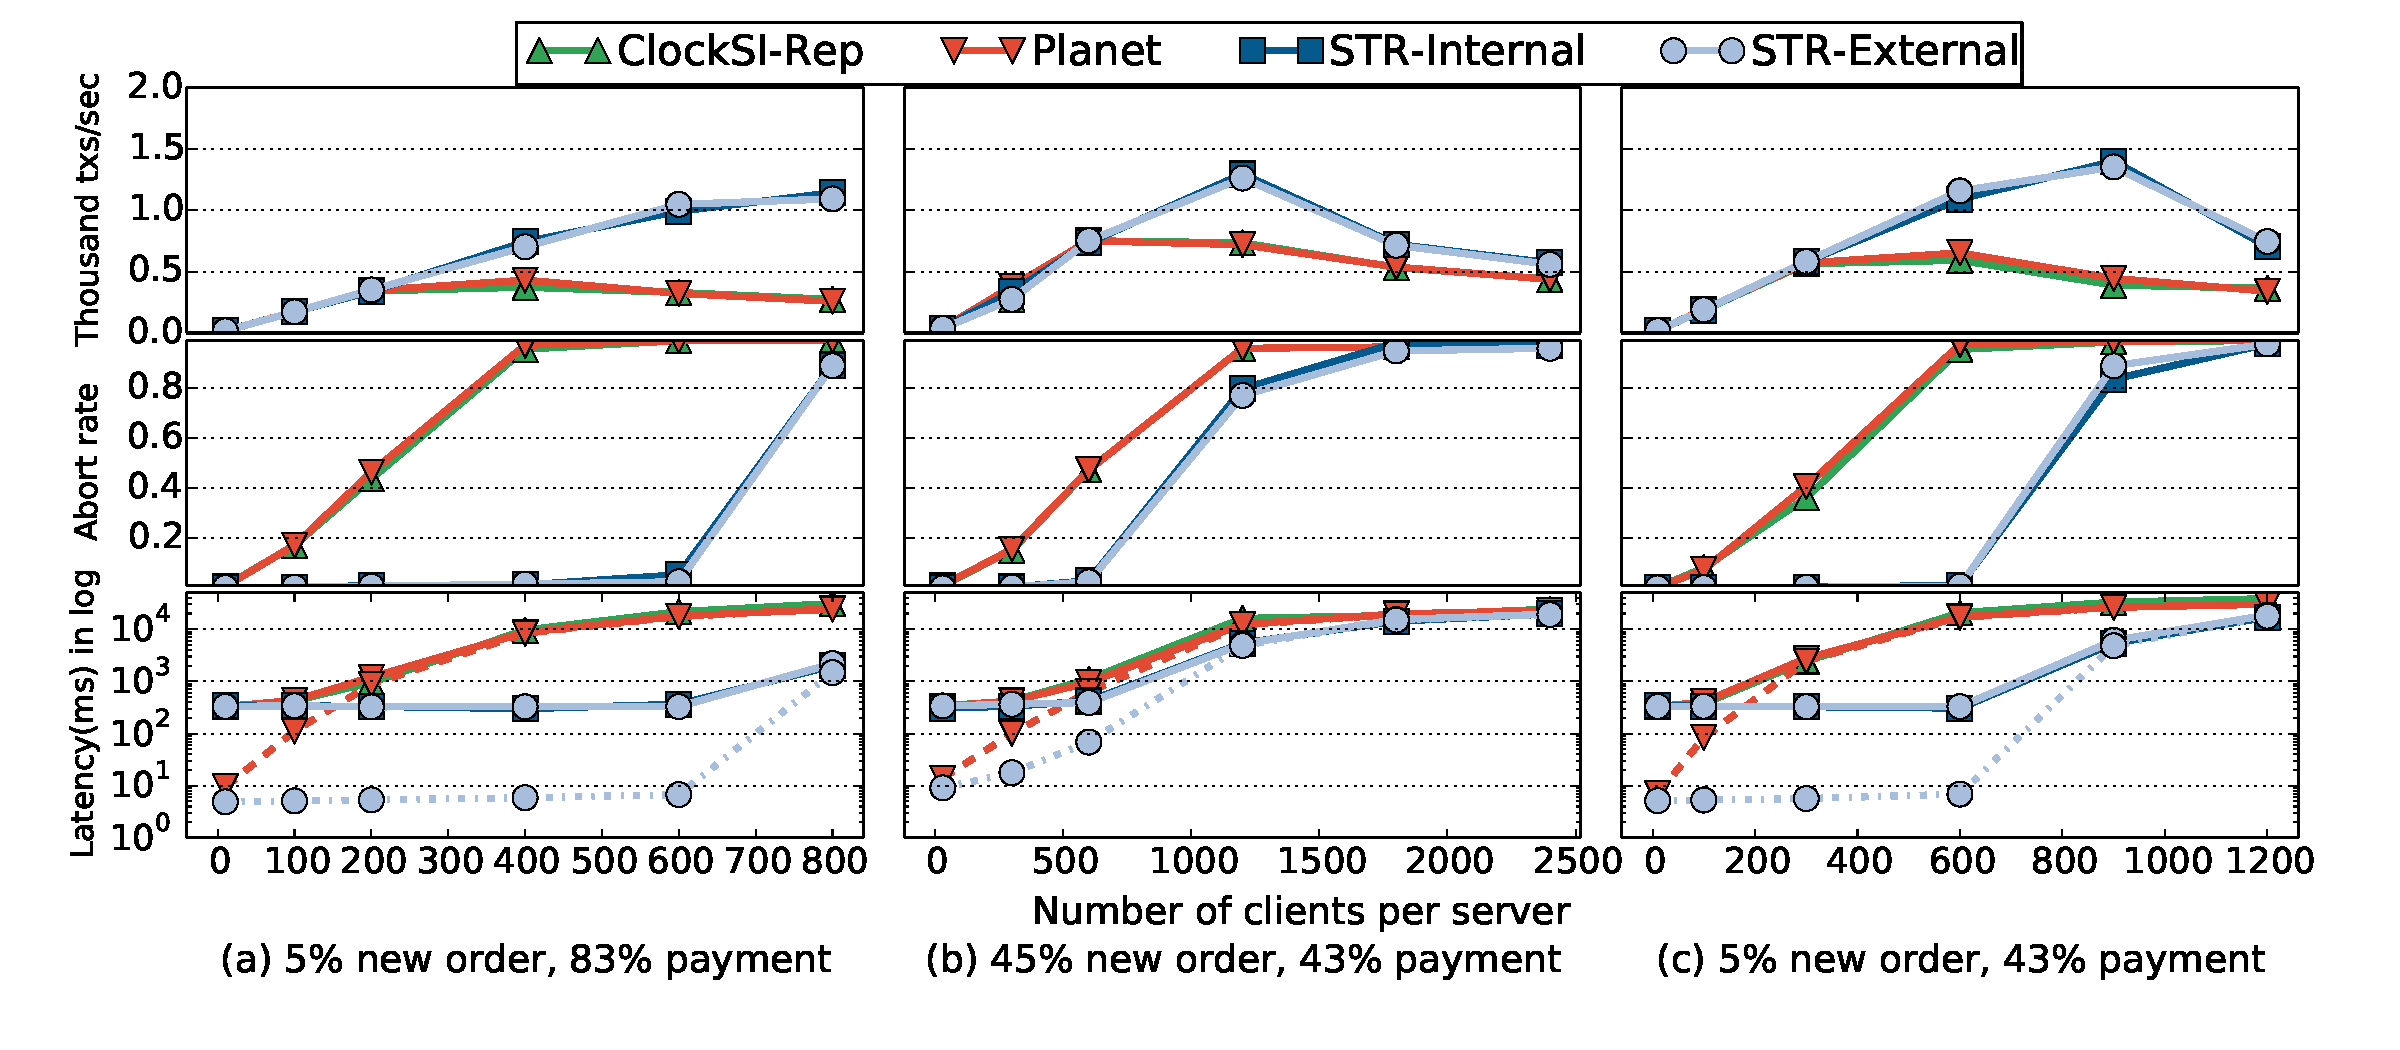
\includegraphics[scale=0.3]{figures/tpcc}
  \vspace{-5mm}
  \caption{\small The performance of different protocols for three TPC-C workloads.}
  \label{fig:tpcc}
\end{minipage}
\begin{minipage}{.26\textwidth}
\centering
  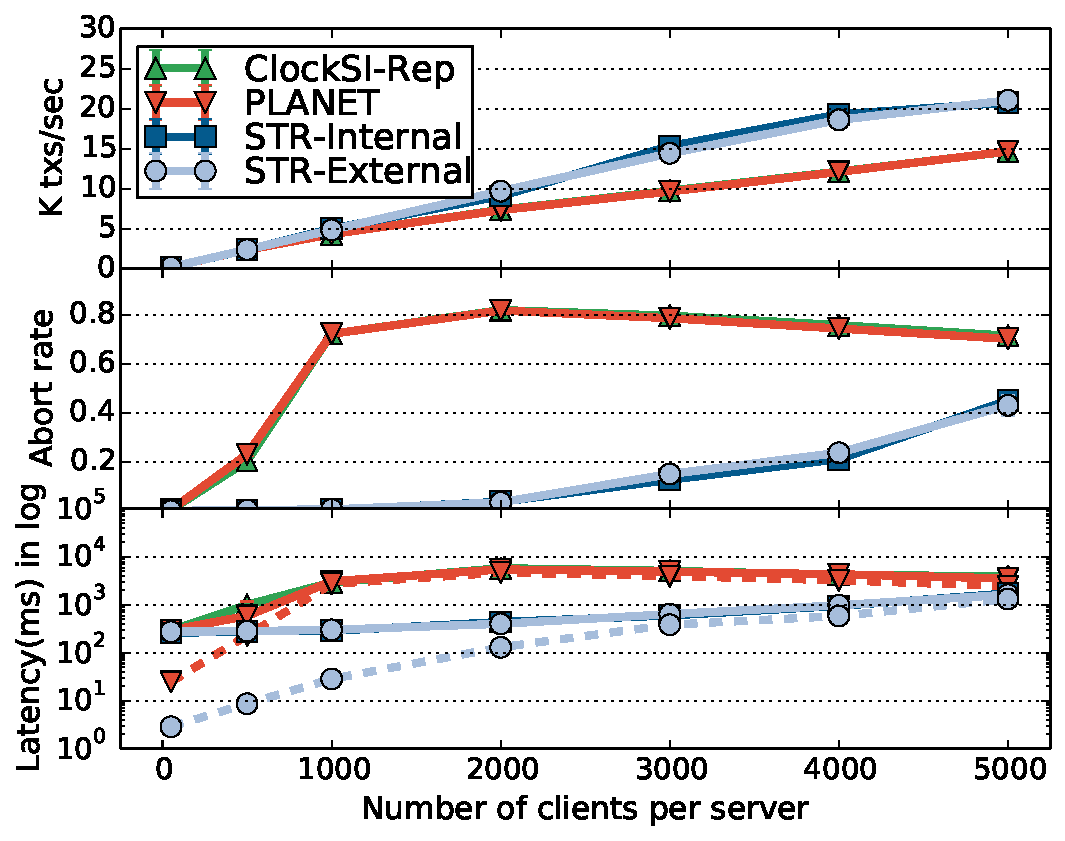
\includegraphics[scale=0.28]{figures/rubislatencywarehouse}
  \vspace{-2mm}
  \caption{\small The performance of different protocols for RUBiS}
  \label{fig:rubis}
\end{minipage}
\end{figure*}


\paragraph{Automatic tuning v.s. static configurations} The previous discussion has shown that \specula's self-tuning mechanism allows for delivering robust performance even in  adverse workload settings. In Figure~\ref{fig:tuning} we report the throughput that \specula would achieve using static configurations of the speculation degree in diverse load and  contention scenarios. The figure shows that the  speculation degree that maximizes throughput varies significantly, and in non-linear ways, as the workload characteristics vary. The data in Figure~\ref{fig:tuning} does not only highlight the relevance of the self-tuning capabilities of \specula. It also provides an experimental evidence of the fact that, once fixed the system's load, the relation between speculation degree and throughput is expressed via convex functions --- a necessary condition to ensure convergence to global optimum for local search strategies such as the one employed by \specula's self-tuning mechanism. This finding supports the design choice of \specula's hill-climbing-based self-tuning strategy, in favour of more complex strategies (like simulated annealing~\cite{hillclimbing}) that sacrifice convergence speed in order to achieve better accuracy in non-convex optimization problems.

% us to design the automatic tuning method. More importantly, as can be seen in the figure, the curve of speculation level to throughput is convex, i.e. if a speculation level gives local maximal throughput, this is guaranteed to be a global maximum throughput. This observation drove the design of the automatic tuning method to be a simple hill climbing algorithm \cite{hillclimbing}: it starts from no speculative read, then proceeds until it finds a local maximal throughput. Despite being simple and fast, this method can reach throughput close to the optimal throughput.



%Reading a key that is not replicated locally causes large latency, which makes it difficult to examine the benefit of speculation. So for most of the experiments, a transaction only accesses keys replicated in local datacenter. We dedicate a separate experiment to examine the effect of remote read on throughput.

\subsection{Macro benchmark}
In the following experiments, we evaluate the performance of \specula with realistic interactive applications, namely TPC-C\cite{tpcc} and RUBiS \cite{rubis}. The key differences between these workloads and the synthetic ones are: (i) while some synthetic workloads already gives severe contention, some transactions of these two applications, e.g. \textit{payment} of TPC-C and \textit{register\_item} of RUBiS, have even more radical contention, which gives \specula better speedup; (ii) to model realistic human to machine interaction, TPC-C and RUBiS specify large ``think time'' between consecutive operations issued by a user, typically a few seconds, which causes speculative commit to not bring obvious performance improvement. Though, speculative commit can still provides low perceived latency.

\subsubsection{TPC-C}
TPC-C \cite{tpcc} models the workload of an online shopping system. We implemented three TPC-C transactions, namely payment, new-order and order-status, according to the specification. Payment transaction has very high local contention and low remote contention; new-order transaction has medium level local and remote contention, and order-status is a read-only transaction. According to the described workload mix rule in the specification, we use three workloads: 5\% new-order, 83\% payment and 12\% order-status (TPC-C A); 5\% new-order, 43\% payment and 52\% order-status (TPC-C B) and 45\% new-order, 43\% payment and 12\% order-status (TPC-C C). We add the ``think time'' and ``key time'' for each transaction as described in the specification, so a client sleeps for some time (from 5 seconds to as large as hundreds of seconds) both before and after issuing a transaction. A server is loaded with five warehouses (more warehouse means less contention), which reaches the server's memory limit.

As we can see in figure \ref{fig:tpcc}, due to having large think time, speculative commit hardly brings any throughput benefit, while speculative read is beneficial due to these workloads all have high local contention. As a result, PLANET achieves the same throughput as ClockSI-Rep, {\specula}-External achieves the same throughput as {\specula}-Internal, and there is a clear throughput difference between STR and the baselines. Though, with low number of clients, PLANET reduces the perceived latency from about 320 millisecond of ClockSI-Rep to about 10 millisecond, by a factor of 32. But when the load increases, the latency of PLANET also increases as local contention is exacerbated. On the other hand, due to allowing speculative read, {\specula}-External and {\specula-Internal} achieve significant speedup compared with the baseline: 2.93$\times$ for TPC-C A, 1.68$\times$ for TPC-C B and 3.47$\times$ for TPC-C C. Both {\specula} protocols also greatly reduce the operation latency by a factor of about 70 compared with the latency of PLANET and ClockSI-Rep.

\subsection{RUBiS}
RUBiS \cite{rubis} models an online bidding system. Of all the 26 user interactions, there are five update transactions: store bid, store buy now, store comment, register item and register user. RUBiS is designed to run on top of a SQL database, so we did the following modification to adapt it to our key-value store: (i) we horizontally partition database tables across servers, so that each server contains an equal portion of data of each table; (ii) many RUBiS insertion operations need to increment a table index to get unique id, which is inefficient when the table is sharded across machines. To avoid this, we let these operations to update local indices that are maintained by local table shards, as studied in \cite{cecchet2008middleware}. We use RUBiS's 15\% update default workload and its default think time (different transactions can have think time from 2 seconds to 10 seconds).

Due to memory limit, we were not able to load the system with more clients. It is hard to saturate servers with TPC-C workloads, because the default workload is dominated by fast read-only transactions and the contention is lower than TPC-C. Nevertheless, the figure \ref{fig:rubis} still shows that \specula achieves good speedup and latency reduction. With 5000 clients, \specula still achieves about 1.43$\times$ speedup compared with ClockSI-Rep and PLANET. Note that the abort rate of PLANET and ClockSI-Rep slightly decreases with increasing number of clients. This is because in RUBiS, the access pattern of a client highly depends on the update of other clients, so with more number of clients, the access pattern gets more diverse and the abort rate is reduced.

